
\documentclass[10pt,a4paper,twocolumn,twoside]{rho-class/rho}
\definecolor{rhocolor}{rgb}{0.0, 0.2, 0.4} % dark blue accent (the template's built-in blue option)
\usepackage[english]{babel}
\usepackage{algorithm}
\usepackage{algpseudocode}
\usepackage{multirow}
\setlength{\columnsep}{0.25in}
\setlength{\intextsep}{6pt}
\setlength{\textfloatsep}{6pt}
\usepackage{titlesec}
\titlespacing*{\paragraph}{0pt}{0.2ex}{0.5em}
\makeatletter
\titlespacing*{\subsubsection}{0pt}{1ex}{2pt}
\makeatother
%----------------------------------------------------------
% Title
%----------------------------------------------------------

\title{DSA5208 Project 2 Report : Scalable Rainfall Forecasting with Apache Spark}

\author{\textbf{Group Members: }Yan Yixin, Zhang Yue, Leon Yiliang Qian}

%----------------------------------------------------------
% Abstract and Keywords
%----------------------------------------------------------

\begin{abstract}

\end{abstract}
\makeatletter
\renewcommand{\rhoabstract}{}
\makeatother

%----------------------------------------------------------
% Footer: page number centred at the bottom of EVERY page, as "n/N"
%----------------------------------------------------------
\makeatletter
% Running head: project title on every page that carries one
\fancyhead[RO,LE]{\footerfont Scalable Rainfall Forecasting with Apache Spark}
\fancyhead[RE,LO]{}
\fancyfoot[C]{\footerfont\thepage/\pageref{LastPage}}
\fancypagestyle{firststyle}{
    \fancyhead[L]{}
    \fancyhead[C]{}
    \fancyhead[R]{}
    \fancyfoot[C]{\footerfont\thepage/\pageref{LastPage}}
    \fancyfoot[L]{
        {\ifx\@journalname\undefined\else\footerfont\bfseries\@journalname\hspace{8pt}\fi}
        {\ifx\@theday\undefined\else\footerfont\@theday\hspace{8pt}\fi}
        {\ifx\@vol\undefined\else\footerfont{Vol.\nobreakspace}\@vol\hspace{8pt}\fi}
        {\ifx\@no\undefined\else\footerfont{No.\nobreakspace}\@no\hspace{8pt}\fi}
        }
    \fancyfoot[R]{
        {\ifx\@journal\undefined\else\footerfont\@journal\hspace{8pt}\fi}
    }
}
\makeatother

\begin{document}

    \maketitle
    \thispagestyle{firststyle}

%----------------------------------------------------------

\noindent\textbf{Submitted material.} The Spark pipeline, the trained model, the generated metric files and the figures reproduced here are submitted together with this report. \textbf{Brief instructions for reproducing the main experiments are given in the accompanying \texttt{README.md}}, which documents the environment, the staged workflow and the controls applied to the experiment runner.

\section{Introduction}
\rhostart{R}ainfall in Singapore is convective, highly localised and fast moving, so a station can pass from dry to heavy rain within a few five-minute intervals. This project asks a question an operational user would ask: given everything observed at a station up to the present moment, what is the probability that the next thirty minutes will accumulate more than a given amount of rain?

We treat this as a probabilistic classification problem over eight years of national observations, built end to end on Apache Spark~\cite{Lecture4}. The work has two halves. The first is an exploratory study of the observation network itself: how complete it is, how rainfall is distributed across months and hours, and which apparent extremes survive scrutiny. The second is a supervised forecasting experiment that compares three MLlib model families against two frequency baselines, selects a model chronologically, and then measures it once on held-out years.

Two commitments shape the whole report. Evaluation is strictly chronological, so no future observation of any kind informs a model that is scored on it. And every quantity reported here is read back from a generated metric file rather than transcribed by hand, so the tables and the experiment cannot drift apart.

\section{Data and Computing Environment}

\subsection{Data Source and Cleaning}
We use the NEA historical rainfall collection published through data.gov.sg~\cite{NEARainfall}, covering 2017 through 2024. Each record carries an observation timestamp, a station identifier, station metadata, coordinates, and a five-minute rainfall total in millimetres. The publisher states that timestamps are Singapore Time, that records may be missing, and that the series has not undergone climate-data quality control. We therefore treat the data as observations, not as a validated climate product.

All processing uses Spark DataFrames~\cite{Lecture4,Lecture5}. Exact semantic duplicates are removed. Where two records disagree for the same station and timestamp, both are excluded rather than arbitrarily resolved. Negative, non-finite, unparseable, geographically invalid and off-grid observations are excluded. Early timestamps falling within one second of the five-minute grid are aligned and audited rather than discarded.

Two cleaning decisions matter for interpretation. Missing observations are never treated as zero rainfall, because an absent reading and a dry reading are different claims. And five-minute values above 50\,mm are retained and flagged rather than removed: that threshold is an engineering audit rule, not a meteorological limit, so silently deleting such values would discard precisely the extremes the study is interested in.

\begin{table}[H]
\caption{Record-level quality audit.}
\label{tab:audit}
\centering
\scriptsize
\setlength{\tabcolsep}{3pt}
\begin{tabular}{lrrrr}
\toprule
\textbf{Year} & \textbf{Raw} & \textbf{Off-grid} & \textbf{Unique valid} & \textbf{Clean} \\
\midrule
2017 & 5\,256\,106 & 1\,775\,327 & 5\,256\,022 & 5\,256\,018 \\
2018 & 4\,594\,246 & 0 & 4\,594\,246 & 4\,594\,246 \\
2019 & 5\,026\,862 & 0 & 5\,026\,862 & 5\,026\,862 \\
2020 & 6\,334\,473 & 0 & 6\,334\,473 & 6\,334\,473 \\
2021 & 7\,044\,646 & 0 & 7\,044\,646 & 7\,044\,646 \\
2022 & 7\,133\,230 & 0 & 7\,133\,230 & 7\,133\,230 \\
2023 & 6\,742\,890 & 0 & 6\,742\,890 & 6\,742\,890 \\
2024 & 6\,406\,260 & 0 & 6\,406\,260 & 6\,406\,260 \\
\bottomrule
\end{tabular}
\tabletext{Note: no invalid records were found in any year. Off-grid counts include observations accepted after one-second alignment, which is why 2017 shows a large count but almost no loss. One station reports more than one distinct coordinate pair across the period; a stable identifier does not guarantee a stable physical location.}
\end{table}

\subsection{Computing Environment}
The reported run was executed on a single machine under WSL2, with Spark in local mode. The configuration is deliberately modest: the point of the exercise is a pipeline that scales by partitioning, not one that depends on a large cluster.

\begin{table}[H]
\caption{Spark runtime configuration for the reported run.}
\label{tab:env}
\centering
\small
\setlength{\tabcolsep}{3pt}
\begin{tabular}{ll}
\toprule
\textbf{Setting} & \textbf{Value} \\
\midrule
Spark & 3.5.3 \\
Python & 3.12.3 \\
Java & 11.0.13 \\
Master & \texttt{local[6]} \\
Driver memory & 4\,g \\
Shuffle partitions & 16 \\
Logical CPUs & 10 \\
RAM & 10.4\,GB \\
\bottomrule
\end{tabular}
\tabletext{Note: platform \texttt{Linux-6.18.33.1-microsoft-standard-WSL2-x86\_64}. Because the whole pipeline runs on one host, elapsed times characterise this machine and are not a scalability benchmark.}
\end{table}

Preparation, which includes cleaning and all exploratory aggregation, took 653.6\,s. Training, which includes the full model comparison and the ablation, took 1517.2\,s.

\subsection{Installation and Reproduction}
The pipeline runs in three stages, \texttt{prepare}, \texttt{train} and \texttt{report}, each invoked through \texttt{run\_experiments.py} and each writing its own log. Raw data, intermediate Parquet and the virtual environment are excluded from version control and are regenerated by the download and preparation commands. The run identifier and the sampling seed are recorded with the outputs, so a later run can be compared against this one rather than silently replacing it.

\section{Prediction Task and Protocol}

\subsection{Target Definition}
For station $s$ and prediction origin $t$, the target is the total rainfall over the next thirty minutes,
\[R_{30}(s,t)=\sum_{k=1}^{6}r(s,t+5k\text{ min}),\qquad y(s,t,a)=\mathbf{1}[R_{30}(s,t)>a],\]
with strict exceedance of threshold $a$. Four thresholds are used: 0, 1, 5 and 10\,mm.

One honest caveat belongs here rather than in the limitations. The published reading type confirms a five-minute total, but the collection does not state whether a timestamp marks the start or the end of its accumulation interval. The target is therefore defined over the next six \emph{recorded} observations; the physical interval-end reading is an assumption we cannot verify from the data.

\subsection{Splits and Sampling}
Training uses 2017--2021, validation uses 2022, and testing uses 2023--2024. Targets that would cross a split boundary are excluded, so no example is partly built from a neighbouring period. A complete example requires twelve past readings from $t-55$ to $t$ and six future readings from $t+5$ to $t+30$. No future observation enters any feature. Encoders, standardisation and baseline probabilities are fitted on training data only.

Of 48\,538\,625 cleaned readings, 47\,048\,853 yield a complete window; window completeness therefore excludes 3.07\,\% of candidate origins.

To keep local computation tractable, training origins are taken every thirty minutes and then sampled uniformly at 10\,\% using a stable hash of station and timestamp with seed 42. The sampling is deliberately origin-level rather than example-level: all four threshold examples derived from a retained origin stay together, so the threshold feature is never correlated with sampling. Validation and testing retain every complete origin, and no class-dependent sampling or reweighting is applied anywhere.

\begin{table}[H]
\caption{Threshold-expanded example counts after completeness, boundary exclusion and training sampling.}
\label{tab:splits}
\centering
\small
\setlength{\tabcolsep}{3pt}
\begin{tabular}{llr}
\toprule
\textbf{Split} & \textbf{Years} & \textbf{Examples} \\
\midrule
Train & 2017--2021 & 1\,796\,204 \\
Validation & 2022 & 4\,714\,860 \\
Test & 2023--2024 & 8\,683\,544 \\
\bottomrule
\end{tabular}
\tabletext{Note: each origin contributes four examples, one per threshold. The training count is smaller than the test count because only training origins are sampled.}
\end{table}

\subsection{Features and Models}
Features are grouped so that their incremental value can be measured rather than assumed.

\begin{table}[H]
\caption{Feature groups; all history ends at the prediction time.}
\label{tab:features}
\centering
\small
\setlength{\tabcolsep}{3pt}
\begin{tabular}{p{0.12\columnwidth}p{0.72\columnwidth}}
\toprule
\textbf{Group} & \textbf{Contents} \\
\midrule
F0 & Station encoding, coordinates, cyclical hour and day-of-year, threshold \\
F1 & F0 plus current five-minute rainfall and six five-minute lags \\
F2 & F1 plus 15/30/60-minute sums, 60-minute maximum, wet count and 15-minute trend \\
\bottomrule
\end{tabular}
\end{table}

A single joint binary classifier is trained with the threshold as a numeric feature, rather than four separate models. This keeps one consistent decision surface and allows other non-negative thresholds to be queried, at the cost that threshold monotonicity is not structurally guaranteed. We measure that property rather than enforcing it.

Three MLlib families are compared~\cite{Lecture6,SparkMLlib}: logistic regression at regularisation 0.01, 0.1 and 1; random forest at 50 and 100 trees with depth 5 and 8; and gradient-boosted trees at 30 and 60 iterations with depth 3 and 5. That is eleven candidates, all sharing identical fitted F2 preprocessing.

\section{Experiment Design}
\label{sec:method}

\subsection{Selection Rule}
Candidates are ranked by validation macro Brier score, averaging the four thresholds equally. Selection uses 2022 only. The test years are never consulted during tuning, and no random cross-validation is used, because shuffling would leak information across time in a series with strong temporal dependence.

Once a winner is chosen, its family and hyperparameters are frozen for the F0/F1/F2 ablation, so that the ablation measures the contribution of features alone rather than a confounded change of model.

\subsection{Baselines}
Two baselines establish what a model must beat to be worth anything. B0 predicts the training exceedance frequency for each threshold, ignoring all inputs. B1 uses training station, month and threshold frequency, falling back to B0 for cells absent from training. B1 is the more demanding comparison: it already encodes the seasonal and spatial structure visible in the exploratory analysis.

\subsection{Evaluation}
The primary metric is the Brier score, which rewards calibrated probabilities rather than confident guesses. Log loss, PR-AUC and ROC-AUC are reported alongside it. PR-AUC is given particular weight at the higher thresholds, where exceedance is rare and ROC-AUC is easy to inflate. Reliability is assessed with ten equal-width probability bins.

For classification metrics, a per-threshold probability cutoff is chosen by maximising validation F1 over 0.05 to 0.95, and then held fixed for the test set.

\section{Results}
All figures below are read from the generated metric files of the reported run. Validation covers 1\,178\,715 origins per threshold; the main test covers 2\,170\,886.

\subsection{Exploratory Analysis}
A station-day enters the daily statistics only when at least 95\,\% of its 288 expected intervals are observed. Annual sums therefore cover qualifying days and are not complete climatological totals.

Across qualifying station-days, November has the highest mean daily rainfall at 10.54\,mm and July the lowest at 5.05\,mm. The maximum wet-interval fraction by month and hour is 0.104, in November at 15:00 SGT, consistent with a convective afternoon peak (Figure~\ref{fig:monthhour}).

\begin{figure}[H]
\centering
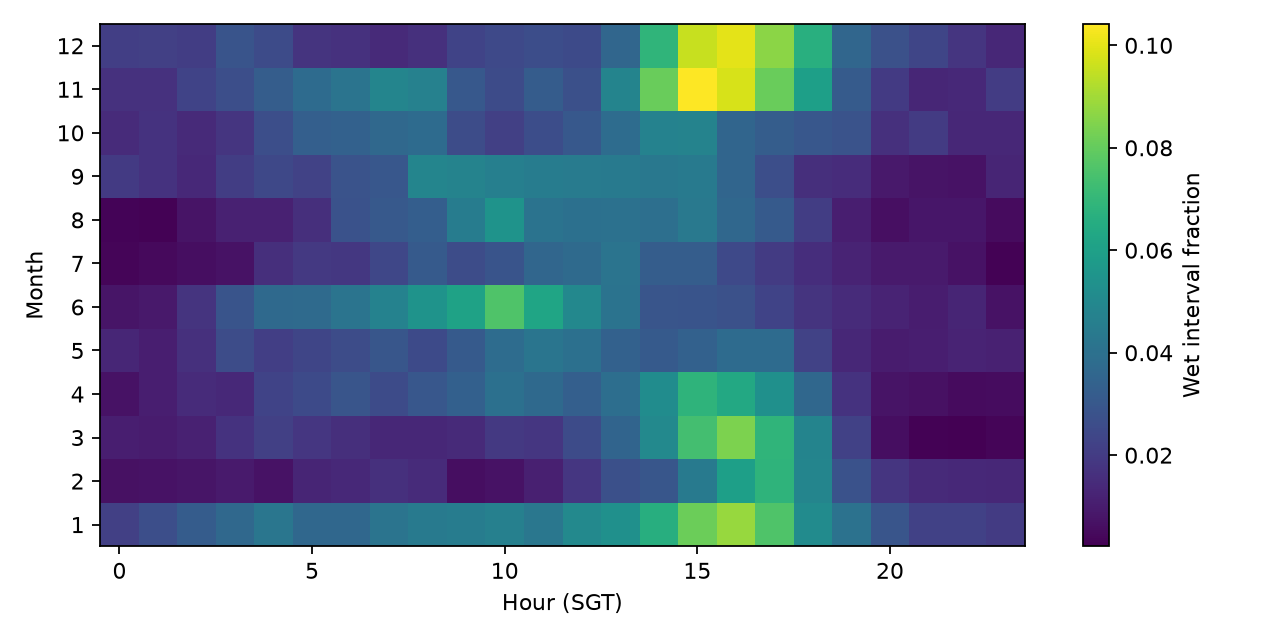
\includegraphics[width=\columnwidth]{month_hour.png}
\caption{Wet-interval frequency by month and local hour. The afternoon peak in the final months of the year is the clearest seasonal structure in the record.}
\label{fig:monthhour}
\end{figure}

Coverage is the limiting factor for any climatological reading. A common-identifier panel of 37 stations has qualifying days in every year, but \emph{no} station achieves 95\,\% full-year coverage in all eight years, so the stricter panel is empty. Comparisons on the common panel therefore control for changing station identifiers but do not eliminate missing-day bias; Figure~\ref{fig:coverage} shows how uneven the coverage is.

\begin{figure}[H]
\centering
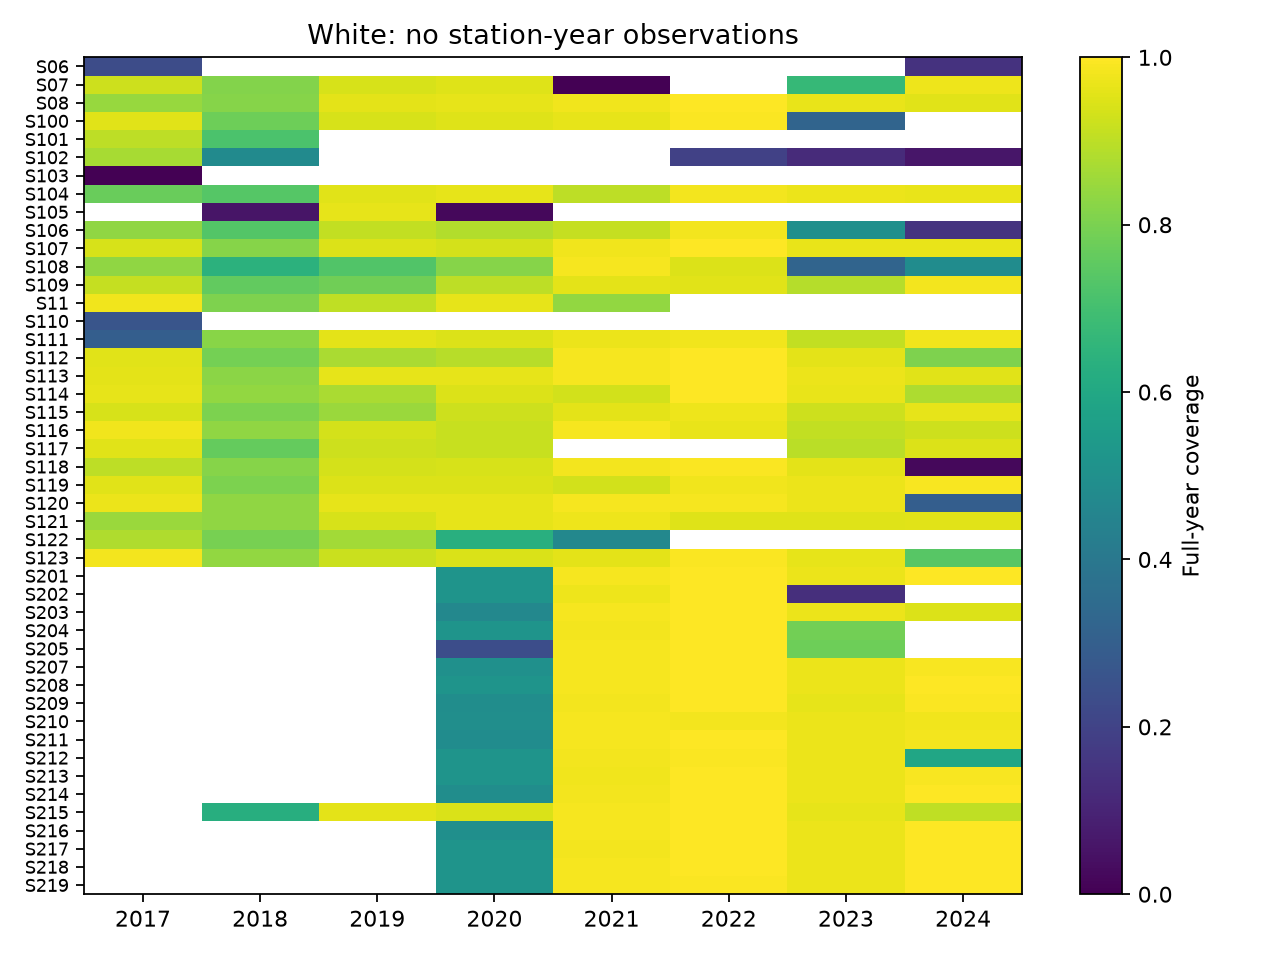
\includegraphics[width=\columnwidth]{coverage_part_1.png}
\caption{Full-year observation coverage by station and year, first panel. White cells carry no observations; the gaps are the reason annual totals are reported as observed sums rather than climatological totals.}
\label{fig:coverage}
\end{figure}

Note also that wet intervals here mean positive observed rainfall, which is not the MSS rainday criterion of at least 0.2\,mm; the two counts are not directly comparable.

\begin{table}[H]
\caption{Largest qualifying station-day totals.}
\label{tab:extremes}
\centering
\small
\setlength{\tabcolsep}{3pt}
\begin{tabular}{llrr}
\toprule
\textbf{Station} & \textbf{Date} & \textbf{mm} & \textbf{Coverage} \\
\midrule
S107 & 2022-08-21 & 786.6 & 0.983 \\
S36 & 2021-04-01 & 319.6 & 1.000 \\
S107 & 2022-08-20 & 262.0 & 0.993 \\
S40 & 2021-08-24 & 247.2 & 1.000 \\
S205 & 2023-02-28 & 210.3 & 1.000 \\
S24 & 2021-01-10 & 205.4 & 1.000 \\
S224 & 2021-01-10 & 197.8 & 1.000 \\
S208 & 2021-01-10 & 197.1 & 1.000 \\
S61 & 2023-02-28 & 196.4 & 1.000 \\
S113 & 2023-02-28 & 194.2 & 1.000 \\
\bottomrule
\end{tabular}
\tabletext{Note: these are observed, unvalidated extremes. The 786.6\,mm total at S107 is far above the others and requires cross-station and provider checks before being treated as a physical record. No positive outlier was silently removed.}
\end{table}

\begin{figure}[H]
\centering
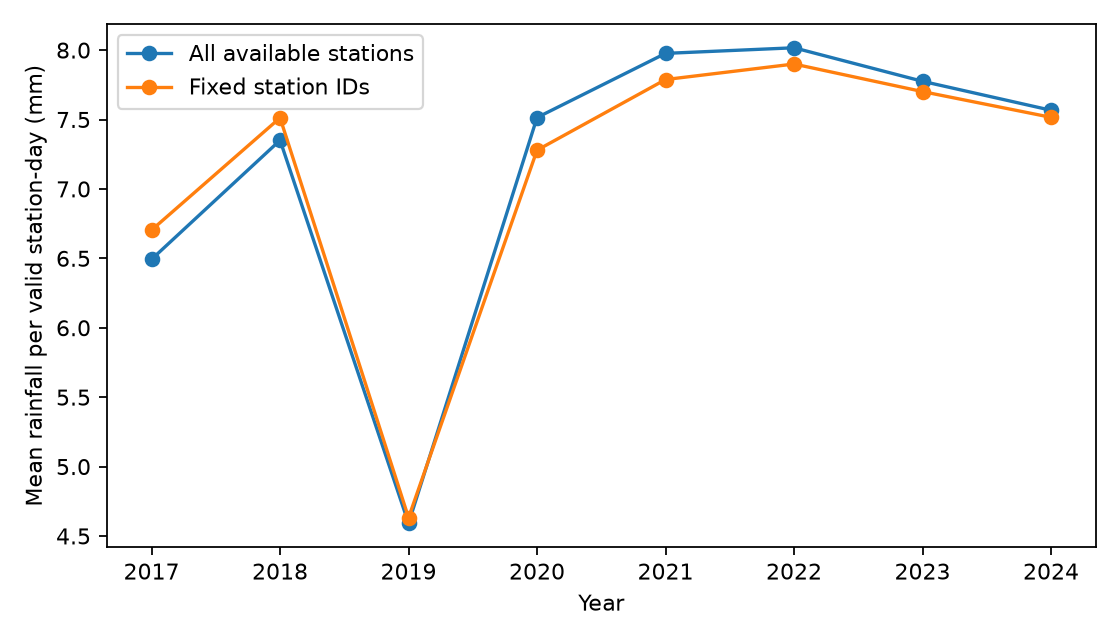
\includegraphics[width=\columnwidth]{annual_daily_mean.png}
\caption{Mean rainfall per qualifying station-day, for all available stations and for the common-identifier panel. The two series track each other closely, so the panel restriction does not materially change the picture.}
\label{fig:annualmean}
\end{figure}

\subsection{Model Selection}
Table~\ref{tab:selection} gives the full comparison. The ordering is clean and unsurprising: logistic regression is worst and degrades monotonically with regularisation; random forest improves with depth rather than with tree count; gradient boosting wins throughout.

\begin{table}[H]
\caption{Chronological validation selection; lower Brier is better.}
\label{tab:selection}
\centering
\scriptsize
\setlength{\tabcolsep}{3pt}
\begin{tabular}{llr}
\toprule
\textbf{Model} & \textbf{Parameters} & \textbf{Macro Brier} \\
\midrule
LR & regParam 0.01 & 0.01871 \\
LR & regParam 0.1 & 0.02097 \\
LR & regParam 1.0 & 0.02327 \\
RF & 50 trees, depth 5 & 0.01752 \\
RF & 50 trees, depth 8 & 0.01609 \\
RF & 100 trees, depth 5 & 0.01774 \\
RF & 100 trees, depth 8 & 0.01632 \\
GBT & 30 iter, depth 3 & 0.01561 \\
GBT & 30 iter, depth 5 & 0.01533 \\
GBT & 60 iter, depth 3 & 0.01493 \\
\textbf{GBT} & \textbf{60 iter, depth 5} & \textbf{0.01474} \\
\bottomrule
\end{tabular}
\tabletext{Note: macro Brier averages the four thresholds equally. Selection used validation year 2022 only.}
\end{table}

The selected model is gradient-boosted trees at 60 iterations and depth 5. Depth matters more than ensemble size: moving random forest from depth 5 to depth 8 improves the score more than doubling the number of trees, which is consistent with the target depending on interactions between recent rainfall and threshold rather than on variance reduction alone.

\subsection{Test Performance}
\begin{table}[H]
\caption{Selected model against baselines, main test origins.}
\label{tab:test}
\centering
\small
\setlength{\tabcolsep}{3pt}
\begin{tabular}{lrr}
\toprule
\textbf{Model} & \textbf{Macro Brier} & \textbf{vs B0} \\
\midrule
B0, global frequency & 0.02472 & --- \\
B1, station/month frequency & 0.02476 & $+0.2\,\%$ \\
GBT, selected & \textbf{0.01461} & $-40.92\,\%$ \\
\bottomrule
\end{tabular}
\tabletext{Note: negative denotes improvement. Each threshold contributes 2\,170\,886 test examples.}
\end{table}

The selected model improves on B0 by 40.92\,\%. The more interesting result is B1: adding station and month structure to the baseline does \emph{not} help, scoring marginally worse than B0 at 0.02476 against 0.02472. Seasonal and spatial climatology alone is close to worthless for a thirty-minute horizon. What matters is the current state of the atmosphere at that station, which is exactly what the ablation below confirms.

Per-threshold behaviour is reported in full in the generated metrics. The pattern is that Brier falls with the threshold simply because exceedance becomes rarer, while PR-AUC falls too, from 0.680 at 0\,mm to 0.250 at 10\,mm. Rare heavy rain remains much harder to anticipate than any aggregate score suggests.

An additional evaluation retains every complete five-minute origin rather than every thirtieth minute, giving 13\,025\,429 origins per threshold and a macro Brier of 0.01460. That the two agree to four decimal places indicates the thirty-minute evaluation stride is not flattering the result. Figures~\ref{fig:calib30} and~\ref{fig:calib5} show the corresponding reliability curves.

\begin{figure}[H]
\centering
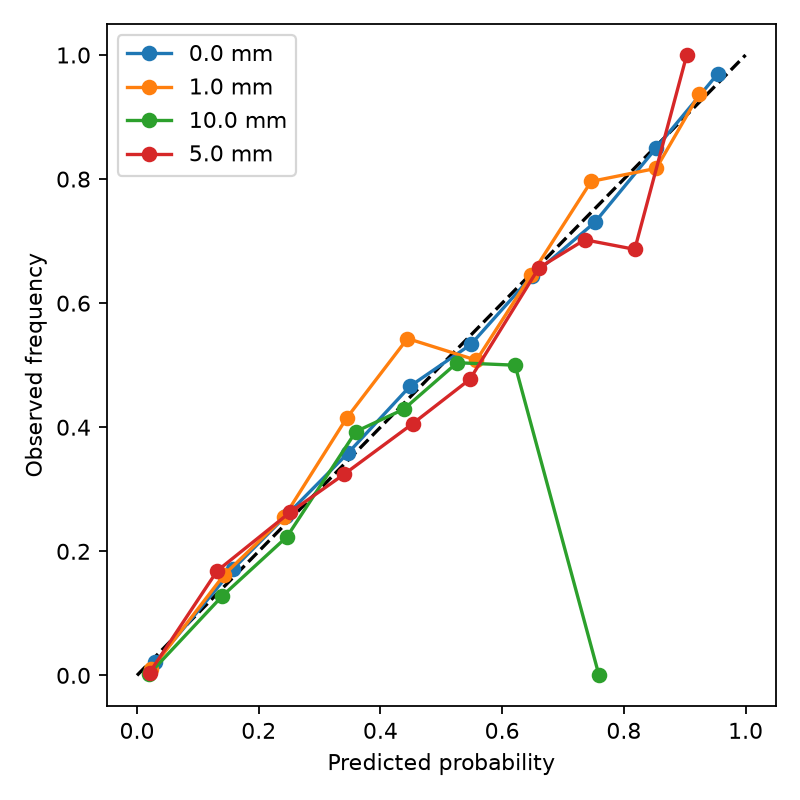
\includegraphics[width=\columnwidth]{test_calibration.png}
\caption{Reliability at 30-minute test origins; the diagonal denotes perfect calibration.}
\label{fig:calib30}
\end{figure}

\begin{figure}[H]
\centering
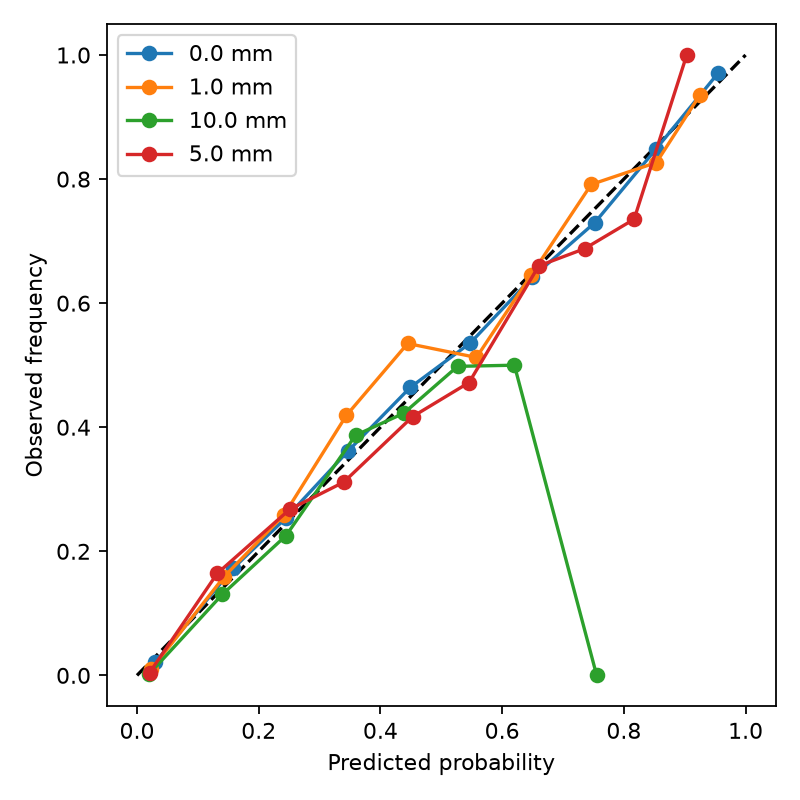
\includegraphics[width=\columnwidth]{five_minute_test_calibration.png}
\caption{Reliability at five-minute test origins, covering 13\,025\,429 origins per threshold.}
\label{fig:calib5}
\end{figure}

\subsection{Feature Ablation}
\begin{table}[H]
\caption{Feature ablation with the winner frozen.}
\label{tab:ablation}
\centering
\small
\setlength{\tabcolsep}{3pt}
\begin{tabular}{lrr}
\toprule
\textbf{Group} & \textbf{Validation} & \textbf{Test} \\
\midrule
F0 & 0.02461 & 0.02441 \\
F1 & 0.01490 & 0.01480 \\
F2 & 0.01474 & 0.01461 \\
\bottomrule
\end{tabular}
\tabletext{Note: macro Brier. Family and hyperparameters are frozen at the selected GBT configuration, so differences reflect features alone.}
\end{table}

This is the clearest result in the study. F0 — station, location, time of day and season, with no rainfall history — scores 0.02441, essentially the baseline level. Adding the current reading and six lags takes it to 0.01480, capturing almost the entire gain. Rolling summaries add a further, much smaller improvement to 0.01461.

In other words, nearly all predictive power comes from knowing whether it is raining right now and how hard. Where and when the station is contributes almost nothing on this horizon.

\subsection{Operating Points and Subgroups}
\begin{table}[H]
\caption{Test classification at validation-selected cutoffs.}
\label{tab:classification}
\centering
\small
\setlength{\tabcolsep}{3pt}
\begin{tabular}{lrrrr}
\toprule
\textbf{mm} & \textbf{Cutoff} & \textbf{Precision} & \textbf{Recall} & \textbf{F1} \\
\midrule
0 & 0.30 & 0.698 & 0.601 & 0.646 \\
1 & 0.25 & 0.651 & 0.535 & 0.587 \\
5 & 0.20 & 0.448 & 0.472 & 0.460 \\
10 & 0.20 & 0.373 & 0.400 & 0.386 \\
\bottomrule
\end{tabular}
\tabletext{Note: cutoffs maximise validation F1 and are then held fixed. They fall as the threshold rises, which is what a well-calibrated model should require for rarer events.}
\end{table}

Conditioning on current state is revealing. Among origins that are currently dry, the model scores 0.0307 at 0\,mm; among origins that are currently wet, it scores 0.0975, with a positive rate of 0.856. The wet subgroup is both much rarer and much harder: once rain has started, predicting whether it continues past a threshold is a genuinely uncertain problem, whereas predicting that dry weather persists is comparatively easy. An aggregate score conceals this, which is why the subgroup breakdown is reported.

Threshold monotonicity, though not enforced, is almost always respected: the probability rises with the threshold in only 1.0 in 10\,000 examples, on both evaluation strides.

Finally, the saved pipeline was reloaded and scored on 20 probe examples, matching the in-memory model to within $10^{-12}$. The eight automated tests covering window exactness, strict exceedance, missing future records, future-feature leakage, temporal boundaries, timestamp alignment and single-class metrics all pass.

\section{Discussion}
\label{sec:disc}

\subsection{What the Results Support}
Three findings are supported by the evidence and are robust to how the evaluation is sliced.

First, short-horizon rainfall exceedance is dominated by persistence. The ablation isolates this cleanly: 96\,\% of the improvement over F0 comes from adding current rainfall and its lags, before any rolling summary is computed. The corollary is that B1 fails — seasonal and spatial frequency, which looks informative in the exploratory analysis, carries almost no thirty-minute predictive signal.

Second, the gain over a frequency baseline is real but bounded. A 40.9\,\% reduction in Brier score is substantial, yet at the 10\,mm threshold precision is 0.373 and PR-AUC is 0.250. The model is useful for ranking risk, not for issuing categorical warnings about heavy rain.

Third, the headline number is not an artefact of the evaluation stride. Re-running on all 13 million five-minute origins moves the macro Brier by 0.00001.

\subsection{What the Results Do Not Support}
The study cannot speak to long-term climate trends. Eight years support descriptive comparison only, and because no station achieves full-year coverage in all eight years, observed annual totals are incomplete by construction.

Nor can it claim operational readiness. Predictions assume every observation through time $t$ is already available; publication latency in the real feed was not measured. A deployment that receives data late would face a harder problem than the one evaluated here.

Finally, the extremes in Table~\ref{tab:extremes} are observations, not validated records. The 786.6\,mm station-day is reported because suppressing it would be worse, not because we are asserting it occurred.

\subsection{Limitations}
\begin{itemize}[topsep=0pt, itemsep=0pt]
\item \textbf{Completeness bias.} Missingness and the 95\,\% coverage filter can bias both the exploratory statistics and the evaluation sample, in directions that cannot be identified from these data alone.
\item \textbf{Unvalidated extremes.} Positive outliers received an audit rule, not external quality control.
\item \textbf{Station identity.} One station reports multiple coordinate pairs; a fixed identifier does not guarantee a fixed location.
\item \textbf{Training sample.} Uniform 10\,\% origin sampling controls computation but discards rare training events, which plausibly costs most at the 10\,mm threshold.
\item \textbf{Generalisation.} The model is assessed on the existing network, not on unseen stations, and non-training thresholds are queryable but not separately validated.
\item \textbf{Dependence.} Adjacent windows and nearby stations are strongly dependent, so no independent-sample confidence intervals are claimed.
\item \textbf{Inputs.} No radar, wind or neighbouring-station features are used; a convective system approaching from an adjacent station is invisible to the model.
\end{itemize}

\section{Conclusion}

\subsection{Conclusion}
This project built a complete Spark pipeline over 48.5 million rainfall observations and used it to forecast thirty-minute exceedance probabilities at four thresholds. Chronological selection across eleven candidates chose gradient-boosted trees at 60 iterations and depth 5, which reached a macro Brier score of 0.01461 on the held-out years 2023--2024, a 40.92\,\% improvement over a frequency baseline.

The most informative result is not the winning score but the ablation. Station identity, location, hour and season together perform at baseline level; adding the current reading and six lags captures almost the entire achievable gain. On a thirty-minute horizon the atmosphere's present state is nearly sufficient, and climatology is nearly irrelevant.

Two caveats travel with that conclusion. The seasonal baseline B1 was no better than the global baseline B0, confirming that the signal is temporal rather than spatial. And performance degrades sharply with rarity: precision falls from 0.698 at 0\,mm to 0.373 at 10\,mm, so the model ranks risk well but should not be read as a warning system for heavy rain.

Within the tested configuration these conclusions are well supported. They do not extend to unseen stations, to real-time operation with publication delay, or to claims about Singapore's rainfall climate.

\subsection{AI Usage Statement}
AI assistants were used at several points in this project, and their roles differed.

OpenAI Codex assisted with the experiment design, the implementation of the Spark pipeline and the generation of an initial automated report. A further draft of the report text was produced with GPT. Anthropic's Claude was used to set up and verify the local environment, to execute the pipeline, and to independently recompute every reported figure from the generated metric files before this report was written.

The group ran the experiments, reviewed the implementation and the results, and is responsible for the final interpretation, the conclusions and the submitted text. Every numerical claim in this report was checked against the preserved metric files rather than copied from a draft.

%======================
% References
%======================

\printbibliography

\end{document}
